\chapter{Introduction}

\akantu means ''little'' element in Kinyarwanda, a
Bantu language. From now on it is also an open source
object-oriented \textit{Finite Element} library which has the ambition
to be generic and efficient.
\akantu is developed within the LSMS (Computational Solid Mechanics Laboratory, \url{lsms.
epfl.ch}), where research is conducted at the interface of mechanics, material
science, and scientific computing. 
The open-source philosophy is important for any
scientific software project evolution. The collaboration
permitted by shared codes enforces sanity when users (and not
only developers) can criticize the implementation details.
\akantu was born with the vision to associate genericity, robustness 
and efficiency while benefiting the open-source visibility.\\

Genericity is necessary to allow the easy exploration of mathematical
formulations through algorithmic ideas. Robustness and reliability
is naturally expected from any simulation software, even more 
in the context of parallel computations. 
In order to achieve these goals, we made noticeable choices in
the architecture of \akantu. First we decided to use the object-oriented
paradigm through C++. Then, in order to prevent extra cost associated 
to virtual function calls we designed the library as
a hybrid architecture with objects at high level layers and
vectorization for low level layers. Thus, Akantu benefits from
inheritance and polymorphism mechanisms without the counter
part of having virtual calls within critical loops. 
This coding philosophy, which was demonstrated in the past to be really 
efficient, is quite innovative in the field of \textit{Finite Element} software. \\

This document is appropriate for people willing to use \akantu
in order to perform a finite element calculation for solid mechanics,
structural mechanics, contact mechanics or heat transfer. The solid mechanics solver, 
that is the most complete and functional part of \akantu, is presented in details throughout 
this document in a step by step approach. 
%If further help should be required 
%requests can be addressed to \href{mailto:akantu@akantu.ch}{akantu@akantu.ch}. 

% \section{Data structures\label{chap:data-structure}}

% \subsection{Vectors\label{sec:vectors}}

% The Vector class is a template class  that can store scalar types as Real, UInt,
% Int  or bool.   A Vector  instance is  defined  by its  size and  its number  of
% component.  It also  has an  identifier and  some extra  internal  variables for
% memory handling purpose.

% \begin{itemize}
% \item The size is the number of tupels stored in the Vector.
% \item The number of component is the number of values stored for each tuple.
% \end{itemize}

% \begin{figure}[!htb]
%   \centering
%   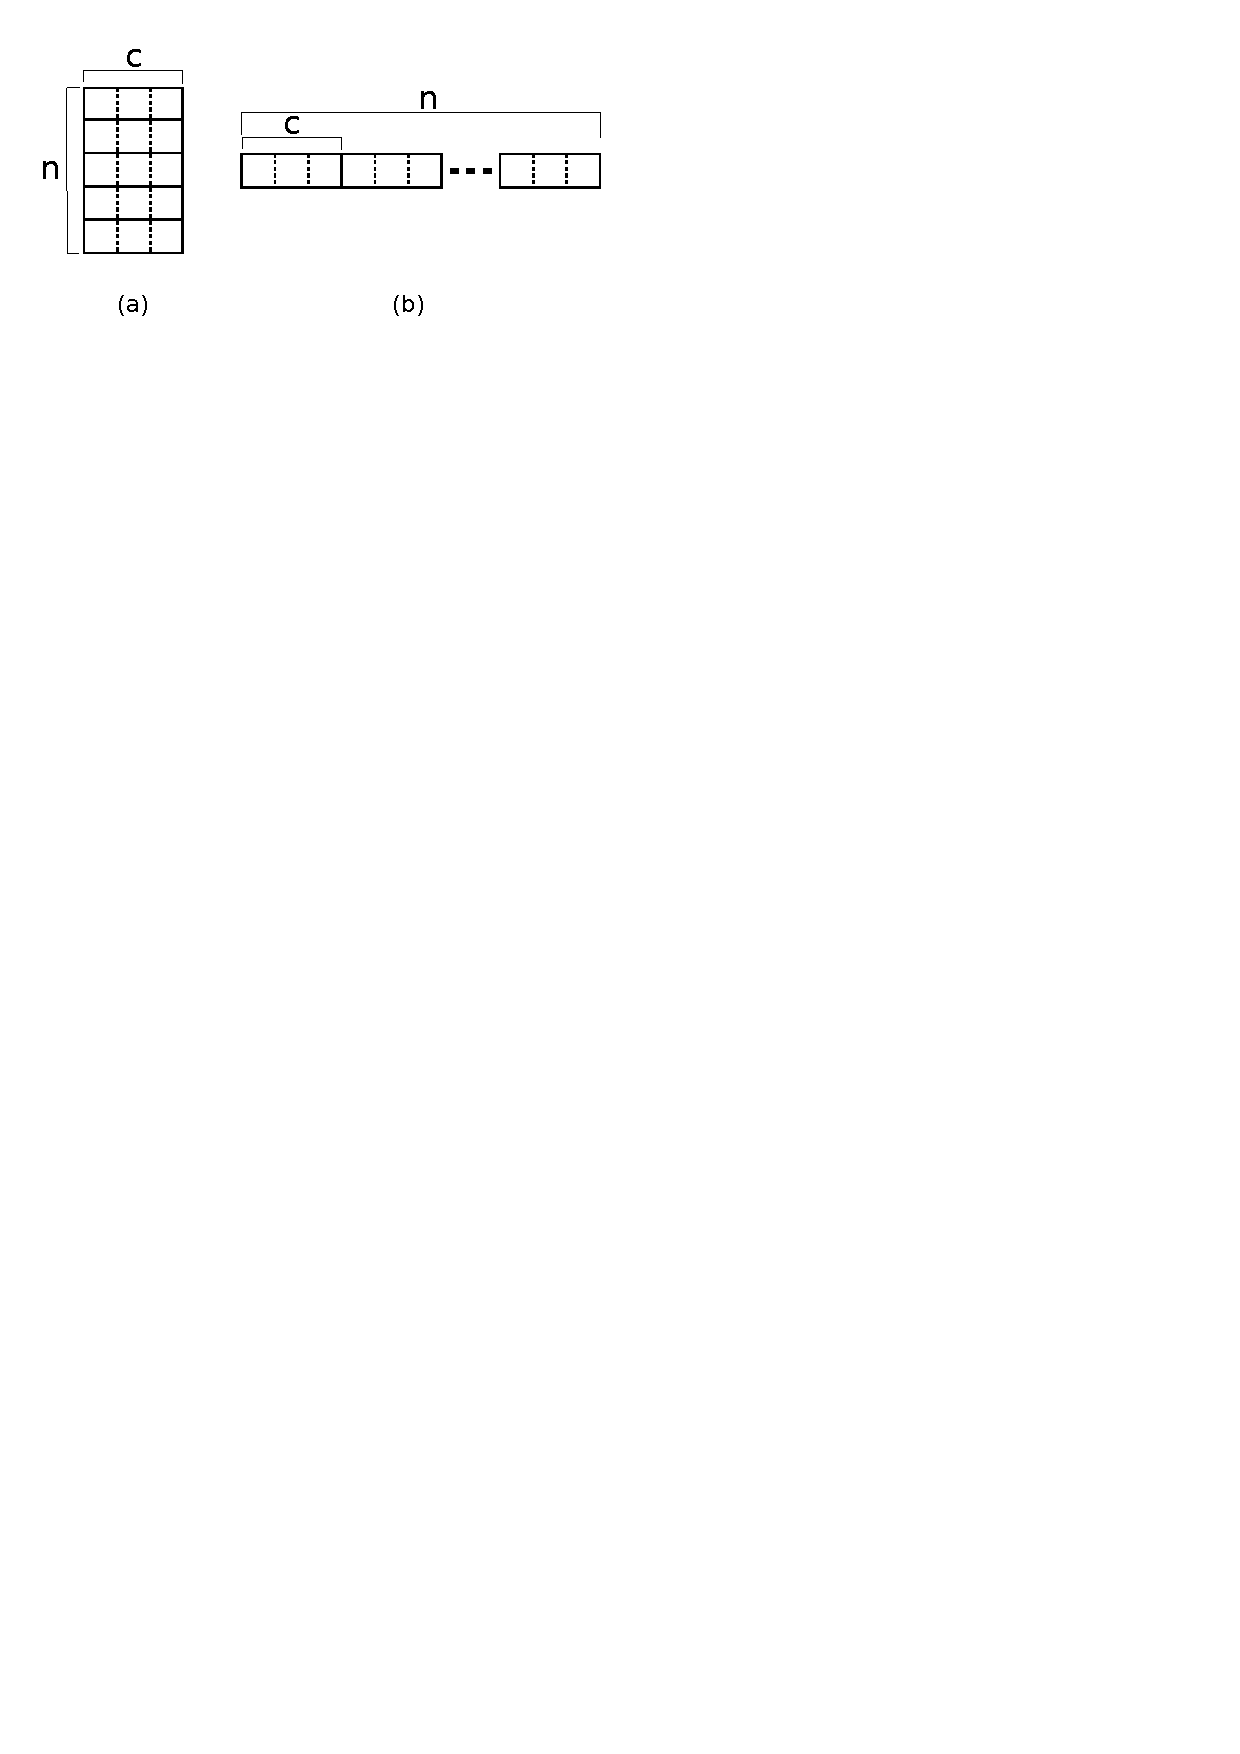
\includegraphics{figures/vectors}
%   \caption{View of  a Vector of size  n and c compenents,  (a) representation of
%     the vector, (b) representation of the storage of the same Vector.}
%   \label{fig:vectors}
% \end{figure}

% All the  data are linerarized  in memory in  an array called values.  This class
% member is public.  So for a Vector  of size $n$ and $c$ component, to access the
% $j^{th}$  component of  th  $i^{th}$ tuple,  you have  to  get $values[i  * c  +
% j]$. You  can also  access to this  value with  accessor \code{at(i, j)}  or the
% constant accessor \code{get(i, j)}.

% If  you want to  store a  matrix on  each tuple  you have  to linearize  it. For
% exemple if you want to store a m * k matrix on each tuple you must specify c = m
% * k.  To access a particular value  in a matrix of  a tuple you will  have to do
% something like $values[ i * m * k + j_i * m + j_j]$.

% \subsubsection{Vector storage convention within FE object\label{sec:FE-convention}}

% The point of  this section is to describe the convention  of storage for vectors
% intented  to be  passed to  {\bf  FE} object  methods.  Indeed  a convention  of
% necessary  since gradient  operators or  integrtaion loops  will use  vectors as
% input and ouput.   Such vectors will be ordered with  a specific convention that
% we intend to describe now.

% For  vector objects,  the  size of  the vector  is  always the  number of  nodes
% associated.  The number  of components  is related  to the  order of  the tensor
% considered. For a scalar  field it is 1, for a vectorial  field, the size of the
% vector is the number of components. For a $m\times n$ matrix field the number of
% components is $m\times n$.

% One common operation  is the manipulation of continuum  fields at the quadrature
% point  positions.   Here  the  size   of  the  vector  is   $mn\_element  \times
% nb\_quad\_points$  and  the  number  of  components is  related  to  the  stored
% object.  For instance the  method \verb$interpolateOnQuadraturePoints()$  take a
% nodal field  stored in a  vector($n\_nodes$,$dim$) and return  a vector($n\_elem
% \times n\_quads$,$dim$).

% Basic gradient operations, like method \verb$gradientOnQuadraturePoints()$, will
% take  as input a  vector($n\_nodes$,$dim$) and  return a  vector($n\_elem \times
% n\_quads$,$dim \times spatial\_dimension$) where spatial dimension is the number
% of dimension in which the domain is embedded.

% In  the  same  way   the  integration  routines  expect  vector($n\_elem  \times
% n\_quads$,$dim$)  and  will  return vector($n\_elem$,$dim$).   For  non-Gaussian
% integrations, the input  by be direction a nodal field.   (At present time, only
% gaussian integrators are implemented within akantu).

% Last but  not the least  is the vectorial  assembly process for which  accept as
% input vector($n\_elem \times n\_quads \times n\_nodes\_per\_element$,$dim$)
% and will return a vector($n\_nodes$,$dim$) nodal object.\\

% {\bf The general convention is that  the number of component shall always be the
%   size of  the object manipulated  at the lowest  level.  The object could  be a
%   per-element, of  per quadrature point  or even per  node basis this  will also
%   apply    as   shown    below.   The    figures    \ref{fig:vector-chain}   and
%   \ref{fig:interpolate-storage} shows the  pattern of the vectors is  the case a
%   interpolation on quadrature points.}

% \begin{figure}
%   \begin{equation}
%     \left(
%       \begin{array}{c}
%         N_1 \\
%         \vdots \\
%         N_I
%         \left\{
%           \begin{array}{c}
%             a_1 \\
%             \vdots \\
%             a_{dim} \\
%           \end{array}
%         \right. \\
%         \vdots \\
%         N_{nb\_nodes}
%       \end{array}
%     \right)
%     \begin{array}{c}
%       \Longrightarrow \\
%       interpolate\\
%       On\\
%       Quadrature\\
%       Points\\
%     \end{array}
%     \left(
%       \begin{array}{c}
%         E_1 \\
%         \vdots \\
%         E_e
%         \left\{
%           \begin{array}{c}
%             q_1 \\
%             \vdots \\
%             \left.
%               \begin{array}{c}
%                 a_1 \\
%                 \vdots \\
%                 a_{dim}
%               \end{array}
%             \right\} q_i \\
%             \vdots \\
%             q_p \\
%           \end{array}
%         \right.  \\
%         \vdots \\
%         E_{nb\_elements}
%       \end{array}
%     \right)
%   \end{equation}
%   \caption{\label{fig:vector-chain}Pattern   of   vectors   manipulated   during
%     interpolation on  quadrature points.  Symbols  N (resp. E, q)  denotes nodes
%     (resp. elements, quadrature points).}
% \end{figure}

% \begin{figure}[!htb]
%   \centering
%   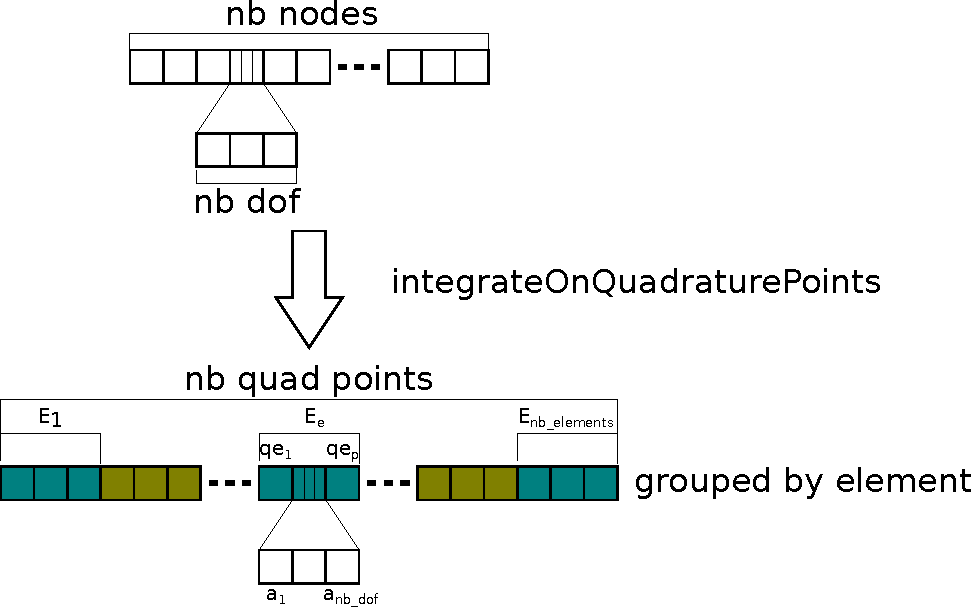
\includegraphics[width=\textwidth]{figures/interpolate}
%   \caption{Input and output  vector of interpolateOnQuadraturePoints. The output
%     Vector has nb\_quadrature\_points tuples,  the quadrature points are grouped
%     by elements (p is the number of quadrature points per element).}
%   \label{fig:interpolate-storage}
% \end{figure}
